\chapter[Autonomes Ladeverhalten]{Autonomes Ladeverhalten \hfill\raggedleft{\normalsize A.G.}} \label{kap:AutonomesLadeverhalten}
Ein wesentlicher Bestandteil von autarken Systemen ist die erwähnte Energieressource. Falls es sich darüber hinaus um ein mobiles System handelt, ist die Verfügbarkeit einer Ladestation auf langer Sicht unabdingbar. Aus diesem Grund muss ein autonomes Ladeverhalten bestehen, welches jederzeit die Ladestation lokalisieren, anfahren und in dieser einparken kann. Dazu ist es bei einem aktuellen Ladevorgang essentiell diesen zu überwachen und zu kontrollieren.

\section[Anfahren der Ladestation]{Anfahren der Ladestation\hfill {\normalsize A.G.}} \label{cha:Anfahren der Ladestation} %TODO: Andi G.
Damit der AMiRo sich in der Ladestation aufladen kann, muss diese zunächst lokalisiert und angefahren werden. Hierbei dient der komplette Schaukasten als Bewegungsfläche und der Schaukastenrand als Begrenzung dieser Fläche. Für die Suche kann der AMiRo auf unterschiedliche Strategien und Verfahren zurückgreifen. Als Suchstrategien existiert zum einen eine Positionsabschätzung über die Kamerabilder der Umgebung, um den kürzesten Pfad zum Schaukastenrand zu berechnen. Zum anderen kann der AMiRo sich in die aktuelle Richtung bewegen und auf gut Glück den Schaukastenrand finden. Als Verfahren zum Anfahren der Ladestation wird entweder auf die Kamera oder auf die Infrarotsensoren am Boden des AMiRo's zurückgegriffen.

In der Abbildung \ref{fig:searchStationFSM} ist die Finite-State-Machine der Lokalisation und des Anfahren der Ladestation als Ablaufdiagramm aufgeführt. Diese lokale State-Machine wird durch die globale Finite-State-Machine angestoßen, welche im Abschnitt \ref{cha:Finite-State-Machine} vorgestellt wird. In der Abbildung wird diese als \texttt{showcaseFSM} beschrieben. Wird das Anfahren der Ladestation aktiviert, beginnt es zunächst aus dem Zustand \texttt{Idle}. Mit der Aktivierung wird eine Information zum weiteren Verlauf mitgegeben. Entweder soll sich der AMiRo zum Schaukastenrand bewegen oder die Ladestation anfahren. Letzteres wird ausgeführt, wenn sich der AMiRo bereits am Schaukastenrand befindet, denn dort muss er bei eventuell besetzter Ladestation warten. Infolgedessen kann die lokale State-Machine in zwei Kernabschnitte betrachtet werden, die im Diagramm als rote Kästen dargestellt sind. Ein beispielhaftes Szenario ist in Abbildung \ref{fig:searchStationExample} visualisiert, wobei der Pfeil zum Schaukastenrand den ersten Kernabschnitt und der Pfeil zur Ladestation den zweiten Kernabschnitt repräsentieren.

\begin{figure}[H]
	\begin{center}
		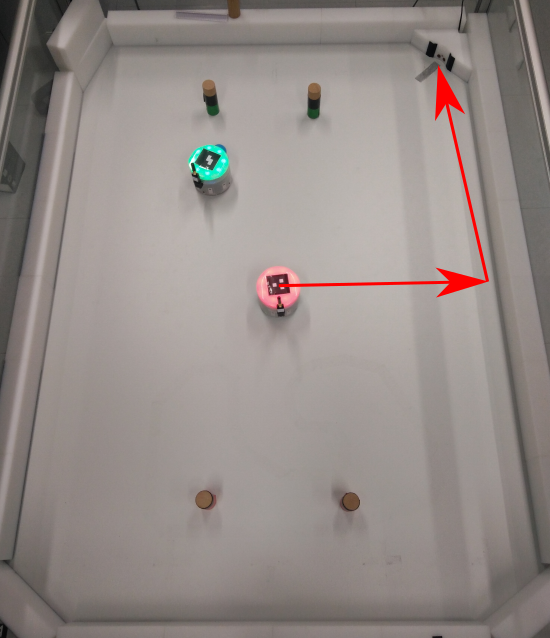
\includegraphics[scale=.45]{searchSationExample.png} 	
		\caption{Aufsuchen der Ladestation}
		\label{fig:searchStationExample}
	\end{center}
\end{figure}

Im ersten Kernabschnitt (oberer roter Kasten in Abb. \ref{fig:searchStationFSM}) soll sich der AMiRo zum Schaukastenrand bewegen. Dabei ruft der Zustand \texttt{Idle} den Zustand \texttt{Initialization} auf. Hier werden für das Lokalisieren und Anfahren Parameter initialisiert und entschieden, welche Suchstrategie ausgeführt werden soll. Soll der AMiRo lediglich in seine aktuelle Orientierung fahren, wird ohne Weiteres der Zustand \texttt{moveAndCollAvoid} aufgerufen. 

Soll hingegen eine intelligentere Suchstrategie angewendet werden, wechselt die State-Machine in den Zustand \texttt{checkPosition}. Der AMiRo rotiert hier einmalig vollständig um seine eigene Achse, während die interne Kamera Bilder von der Umgebung aufnimmt. Über die Bilder läuft der \textit{SimpleBlobDetector} der OpenCV-Programmbibliothek, wobei das Bild zunächst vorverarbeitet wird. Bei der Vorverarbeitung wird pixelweise entschieden, ob der aktuelle Bildpunkt in einem bestimmten Farbwertrahmen fällt oder nicht. Bei zutreffender Bedingung erhält er eine bestimmte Farbe, andernfalls wird er weiß eingefärbt. Damit bietet es dem \textit{SimpleBlobDetector} eine kontrastreiche Vorlage, um Elemente im Kamerabild zu detektieren. Wurde ein Torpfostenpaar und optional die Ladestation detektiert, werden zum einen jeweils die Orientierung der Odometrie abgespeichert. Zum anderen werden jeweils Minimum und Maximum der X- und Y-Koordinaten beider Torpfosten bestimmt. Mit diesen Informationen wechselt die State-Machine in den Zustand \texttt{goalDetected}, ansonsten direkt in den Zustand \texttt{moveAndCollAvoid}.

\begin{figure}[H]
	\begin{center}
		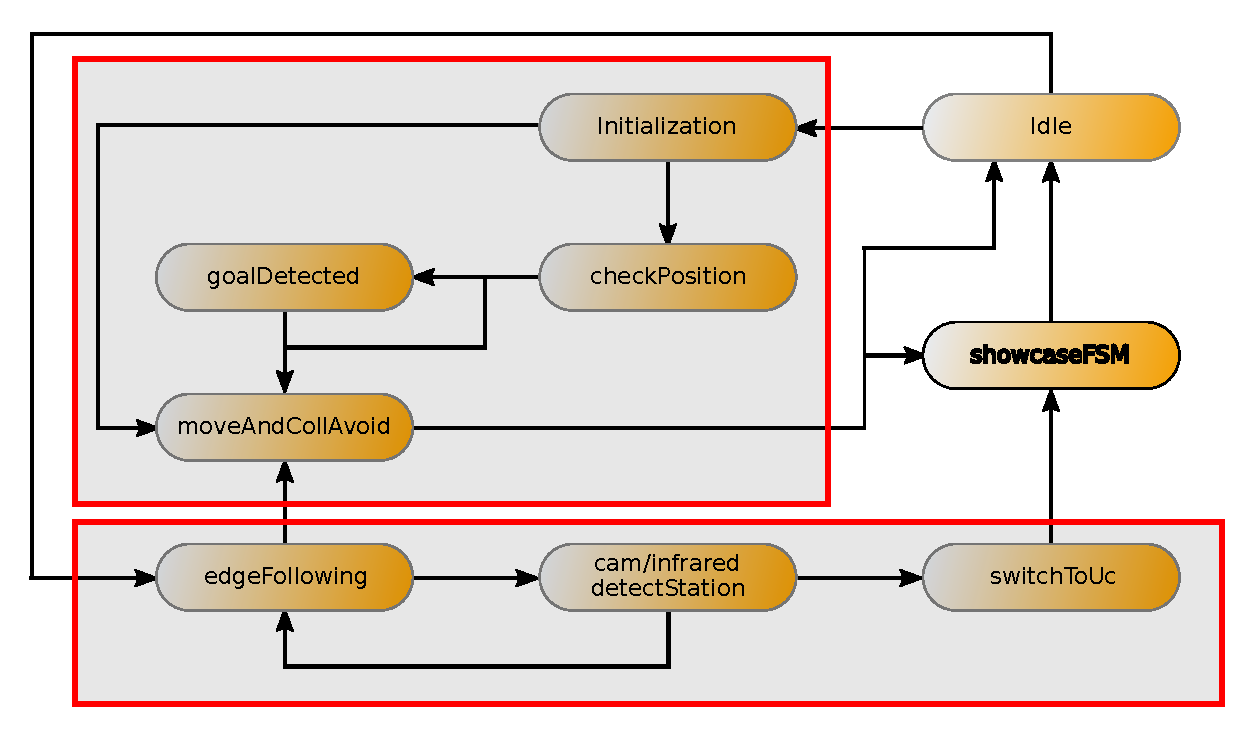
\includegraphics[scale=.7]{searchStationFSM.pdf} 	
		\caption{Finite-State-Machine zum Anfahren der Ladestation}
		\label{fig:searchStationFSM}
	\end{center}
\end{figure}

Das Vorgehen zur Berechnung der nächsten Kante in \texttt{goalDetected} wird in Abschnitt \ref{cha:Lokalisation der Ladestation} erläutert. Nachdem sich der AMiRo zur nächsten Kante orientiert hat, wird ebenfalls der Zustand \texttt{moveAndCollAvoid} aufgerufen. In diesem Zustand bewegt sich der AMiRo geradeaus, entweder eine definierte oder unbegrenzte Strecke. Im ersteren Fall wird eine neue Position angefahren, da die Detektion der Torpfosten an der alten Position nicht erfolgreich war. Damit wechselt die State-Machine in den Zustand \texttt{Idle} und beginnt von vorne. Die Anzahl der Versuche ist hierbei einstellbar, sodass der AMiRo zur Not die aktuelle Orientierung anfährt. Dies entspricht dem zweiten Fall, der unbegrenzten Strecke. Mit einer Kollisionsvermeidung wird anschließend das aktuelle Hindernis vorerst als Schaukastenrand interpretiert. Damit endet der erste Kernabschnitt der lokalen State-Machine und sendet ein Signal an die \texttt{showcaseFSM}.

Der zweite Kernabschnitt (unterer roter Kasten in Abb. \ref{fig:searchStationFSM}) befasst sich mit dem Anfahren der Ladestation. Dazu wird ausgehend vom Zustand \texttt{Idle} mit der Information der \texttt{showcaseFSM} der Zustand \texttt{edgeFollowing} angestoßen. Die durchzuführende Kantenverfolgung ist in Abbildung \ref{fig:edgeFollowing} dargestellt. Ausgehend von einer erfolgreichen Detektion der Ladestation im ersten Kernabschnitt, wird zunächst die Richtung der Kantenverfolgung gesetzt. Das bedeutet den kürzesten Pfad zur Ladestation entweder im oder gegen den Uhrzeigersinn. Des weiteren wird mithilfe der Infrarotsensoren seitlich am AMiRo versucht einen bestimmten Abstand zum Schaukastenrand einzuhalten. Hierbei wird permanent überprüft, ob die Sensoren einen minimalen oder maximalen Schwellwert überschreiten. Trifft dies zu, wird ein entsprechender Rotationswert (links/rechts) angelegt. Befindet sich der Sensorwert zwischen min. und max. Schwellwert, bewegt sich der AMiRo geradeaus. Parallel wird die Orientierung der Odometrie zur Kantenüberprüfung aufsummiert. Erreicht die Summe einen zu hohen Wert, befindet sich der AMiRo nicht an der Kante, da die Innenwinkelsumme eines Rechteckes $360^\circ$ beträgt. Damit wechselt der Miniroboter zurück zum Zustand \texttt{moveAndCollAvoid} und sucht ein neues Hindernis bzw. Kante.

Nachdem Motorwerte zur Kantenverfolgung gesetzt sind, wechselt die State-Machine in den Zustand \texttt{cam/infrared detectStation}. An dieser Stelle wird ein Verfahren zur Detektion der Ladestation verwendet, mittels Kamera oder Infrarotbodensensoren.

\begin{figure}[H]
	\begin{center}
		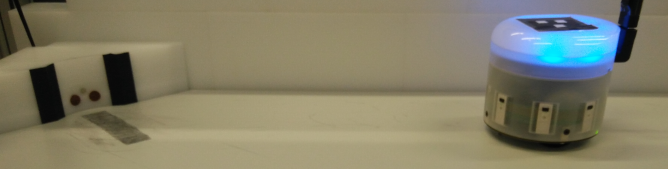
\includegraphics[scale=.6]{edgeFollowing.png} 	
		\caption{Kantenverfolgung und Anfahren der Ladestation}
		\label{fig:edgeFollowing}
	\end{center}
\end{figure}

Die Detektion über das Kamerabild verläuft sehr ähnlich zur Detektion der Torpfosten im ersten Kernabschnitt. Wiederholt wird das Kamerabild vorverarbeitet und der \textit{SimpleBlobDetector} zur Erkennung der schwarzen Markierungen der Ladestation verwendet. Sind keine passenden Elemente detektiert worden, wechselt die State-Machine zurück in den Zustand \texttt{edgeFollowing}. Dies geschieht solange in einer Schleife, bis beide schwarzen Markierungen detektiert worden sind. Ab diesem Punkt richtet sich der AMiRo mit dem Bildmittelpunkt (X-Achse) zur Ladestation aus und fährt sie direkt an. Weiterhin, im aktuellen Zustand verweilend, wird durchgängig über die seitlichen Infrarotsensoren der Abstand vor dem Miniroboter überprüft. Durch die Überschreitung eines Schwellwertes befindet sich der AMiRo anschließend in der Ladestation und wechselt zum Zustand \texttt{switchToUc}.

Ein zweites Verfahren ist die Detektion über die Infrarotbodensensoren. In Abbildung \ref{fig:edgeFollowing} ist eine schwarze Bodenmarkierung an der Ladestation ersichtlich. Wie bei der Detektion mit dem Kamerabild, wechselt die State-Machine solange zwischen diesem Zustand und dem Zustand \texttt{edgeFollowing}, bis die Infrarotsensoren am Boden einen Schwellwert überschreiten. An dieser Stelle wird die Geschwindigkeit gedrosselt und der AMiRo richtet sich zur Ladestation aus. Sobald die seitlichen Bodensensoren die schwarze Fläche detektieren, wird der Miniroboter nochmals zur Ladestation ausgerichtet. Des weiteren bewegt er sich langsam zur Station und sobald die vorderen (Ringsensoren) einen Schwellwert überschreiten, befindet sich der AMiRo in der Ladestation und wechselt zum Zustand \texttt{switchToUc}.

Der Zustand \texttt{switchToUc} ist der finale Zustand in dieser State-Machine. Hier werden Parameter zurückgesetzt und das erfolgreiche Anfahren der Ladestation durch Lichter visualisiert. Ein Signal an \texttt{showcaseFSM} beendet den zweiten Kernabschnitt.

\section[Lokalisation der Ladestation durch Positionsabschätzung]{Lokalisation der Ladestation durch Positionsabschätzung\hfill {\normalsize A.G.}} \label{cha:Lokalisation der Ladestation}
Da der Begriff \textit{autonom} ein gewisses intelligentes Verhalten für die Selbstständigkeit mit sich zieht, ist eine zufällige Suche der Ladestation nicht optimal. Aus einer Menge vieler möglichen Strategien wurde die Berechnung der nächsten Kante und die darauffolgende kürzeste Strecke zur Ladestation gewählt. Diese Strategie lässt sich gut über das Kamerabild realisieren und bietet durch die Aufteilung eine Robustheit mit der Annahme, dass die Ladestation durch eine Kantenverfolgung erreicht werden kann.

Da im Schaukasten hinsichtlich der Markierungen sehr minimalistisch gearbeitet wurde, ist eine Positionsabschätzung anhand der Torpfosten eine gute Möglichkeit. Alternativ wäre eine interne Karte eine weitere Möglichkeit, allerdings ist dies im Rahmen dieses Projektes ein zu hoher Aufwand.

Mit der Bestimmung des nächsten Torpfostens beginnt der Zustand \texttt{goalDetected}. Grundlage dafür sind die über den \textit{SimpleBlobDetector} jeweils ermittelten minimalen und maximalen X- und Y-Koordinaten der Torpfosten. Mit der Annahme, dass Objekte mit zunehmender Entfernung zum Betrachter kleiner wirken, wird der nächste Torpfosten anhand der relativen Größe bestimmt. Diese Information ist im späteren Verlauf für die endgültige Ausrichtung wichtig. Als nächstes folgt die vorläufige Drehung zum Tor, um die einzelnen Schritte zu visualisieren. Dies wird in der Abbildung \ref{fig:firstRotationToPost} dargestellt. Die Orientierung der Odometrie zum Tor wurde in der vorherigen Detektion der Torpfosten mit abgespeichert (rote, gestrichelte Linie). Der Differenzwinkel $\Delta_\Theta$ wird aus dieser und der Orientierung der Startposition berechnet.

\begin{figure}[h]
	\begin{center}
		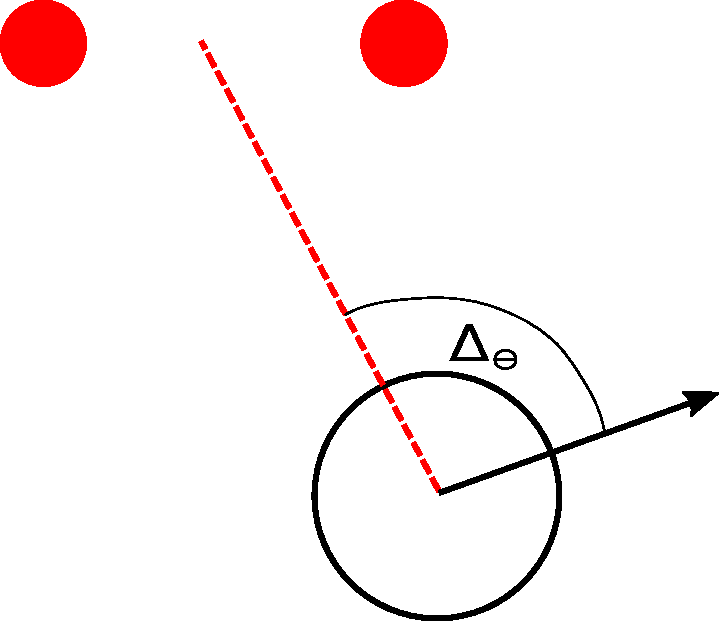
\includegraphics[scale=.5]{firstRotationToPost.pdf} 	
		\caption{Ausrichtung des AMiRo zum Tor}
		\label{fig:firstRotationToPost}
	\end{center}
\end{figure}

Mit den statischen Informationen der Torpfosten (Position und Dimensionen), können diese als Landmarken im Raum verwendet werden. Die Schaukastendimensionen dienen dazu als Koordinatensystem, um eine Positionsabschätzung zu liefern. Dafür werden im folgenden die Distanzen zu den Torpfosten und die Winkel zu diesen benötigt, die mittels Trigonometrie berechnet werden.

Die Distanzberechnung zum Torpfosten ist schematisch in Abbildung \ref{fig:distToPost} dargestellt. Hierbei ist der Winkel $\Theta$ der halbe vertikale Kamerawinkel, da im gesamten Verlauf die relevanten Objekte unterhalb des Horizontes liegen und nur das untere Kamerabild betrachtet wird. Dies spart zum einen Rechenleistung bei der Bildanalyse und zum anderen reduziert es potentiell falsche Objektdetektion. Um die Gegenkathete $B$ zu erhalten, wird die statische Größe des Torpfostens auf die vertikale Bildgröße hochskaliert. Mit Winkel $\Theta$ und Gegenkathete $B$ wird in der Gleichung \ref{eq:distanceToPost} die Ankathete bzw. Distanz $A$ bestimmt.

\begin{figure}[h]
	\begin{center}
		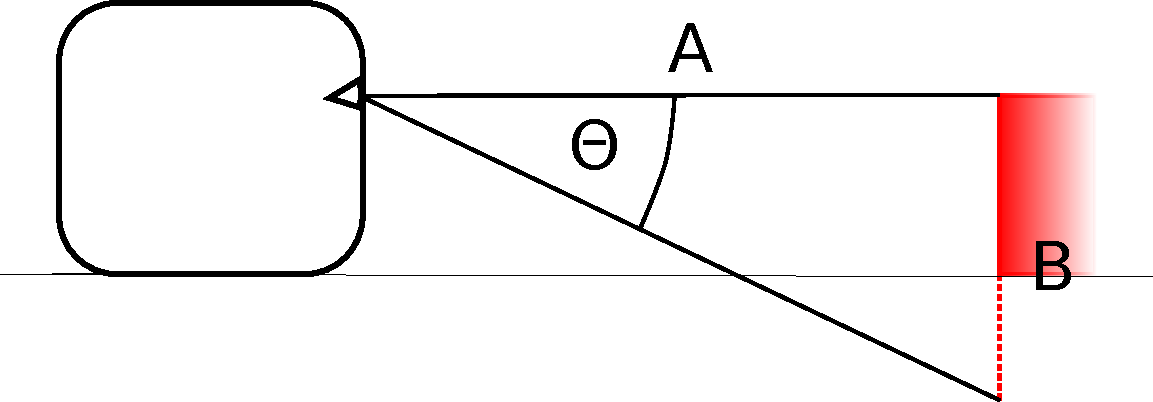
\includegraphics[scale=.5]{distanceToPost.pdf} 	
		\caption{Distanzberechnung zum Torpfosten}
		\label{fig:distToPost}
	\end{center}
\end{figure}

\begin{equation}
	A = B \cdot \tan(\Theta)
	\label{eq:distanceToPost}
\end{equation}

Für die Berechnung der Positionswinkel zu dem Torpfosten wird der Kosinussatz verwendet. Hierzu sind in Abbildung \ref{fig:trianglePost} die zuvor berechneten Distanzen zu den Torpfosten als Ankathete $B$ und Hypotenuse $C$ zu sehen. Der Gegenkathete $A$ ist der Abstand zwischen den Torpfosten und somit eine bekannte Konstante. Mit den drei Seiten können alle Winkel des Dreiecks über den Kosinussatz, den Gleichungen in \ref{eq:anglePost}, berechnet werden. Der relevante Positionswinkel ist hier die Summe $\epsilon = \alpha + \beta$. Steht der AMiRo linksseitig vom Tor, wäre die Winkelsumme $\epsilon = \alpha + \gamma$ (nächster Torpfosten, siehe oben). 

\begin{equation}
	\begin{aligned}
		\alpha = \arccos(\frac{B^2 + C^2 - A^2}{2 \cdot B \cdot C}) \\\\
		\beta = \arccos(\frac{A^2 + C^2 - B^2}{2 \cdot A \cdot C}) \\\\
		\gamma = \arccos(\frac{A^2 + B^2 - C^2}{2 \cdot A \cdot B})
		\label{eq:anglePost}
	\end{aligned}
\end{equation}

\begin{figure} []
	\subfigure[Winkelberechnung]{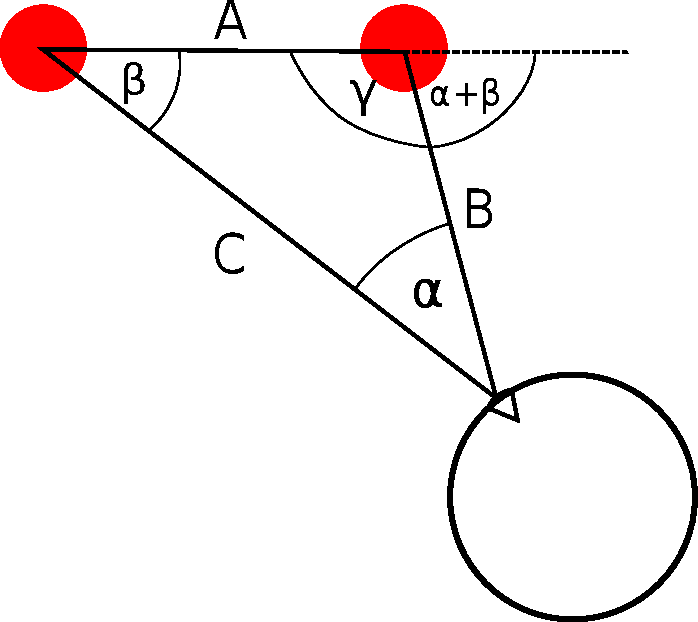
\includegraphics[width=0.4\textwidth]{trianglePost.pdf}\label{fig:trianglePost}} \hspace{2cm}
	\subfigure[Koordinatenberechnung]{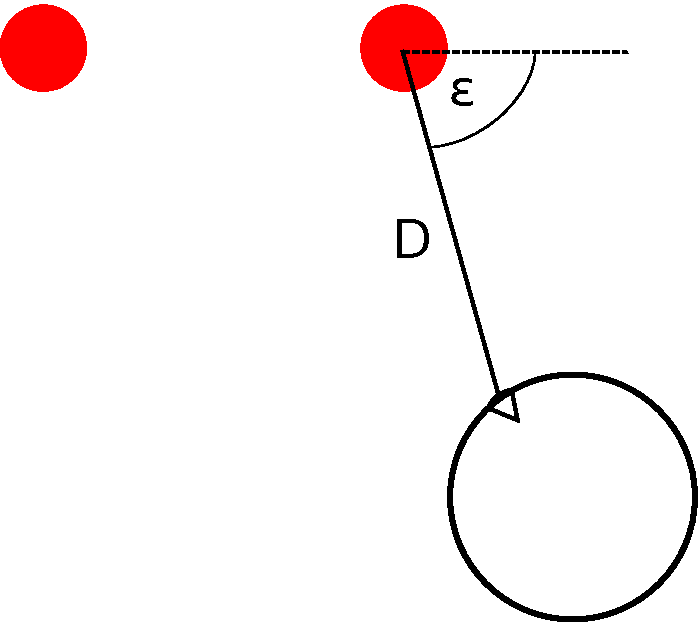
\includegraphics[width=0.4\textwidth]{coordsAmiro.pdf}\label{fig:coordsAmiro}} 
	\caption{Winkel- und Koordinatenberechnung des AmiRo} 
	\label{fig:triangleAndCoordsPost}
\end{figure}

Durch die hinzugekommenen Distanz- und Winkelinformation ist nun eine Positionsabschätzung möglich. In Abbildung \ref{fig:coordsAmiro} sind diese eingezeichnet. Die beiden Gleichungen in \ref{eq:positionCoords} beschreiben die Berechnung der X und Y Koordinaten mit $D$ als Distanz und $\epsilon$ als Winkel. Abhängig von der Position des AMiRo's zum nächsten Torpfosten, linksseitig oder rechtsseitig, wird der Wert zur Torposition addiert oder subtrahiert.

\begin{equation}
	\begin{aligned}
		x\_amiro = x\_tor~+-~~D \cdot \cos(\epsilon) \\
		y\_amiro = y\_tor~+-~~D \cdot \sin(\epsilon)
		\label{eq:positionCoords}
	\end{aligned}
\end{equation}

Mit der Positionsabschätzung lässt sich im Weiteren die nächste Kante identifizieren. In der Abbildung \ref{fig:showcaseSplit} ist die Aufteilung der Fläche des Schaukastens ersichtlich. Jedes Gebiet beschreibt dabei die Richtung zur nächsten Kante, welche durch die vier großen Pfeile in der Abbildung verdeutlicht wird. Da der Schaukasten als Koordinatensystem angesehen wird und dem AMiRo eine Positionsabschätzung mit Koordinaten zugeordnet wurde, kann das aktuelle Gebiet ermittelt werden. Der Positionswinkel $\epsilon$ wird hier als Grundlage zur Ausrichtung zur nächsten Kante eingesetzt. Dieser Winkel $\epsilon$ beschreibt in diesem Szenario immer ein Drehwinkelverhältnis zu einem der seitlichen Kante. Das bedeutet den tatsächlichen Drehwinkel $\Delta_\Theta = 180 - \epsilon$, welcher dem Winkel $\gamma$ aus der Abbildung \ref{fig:trianglePost} entspricht. In $90^\circ$-Schritten wird der Drehwinkel für die anderen Kanten ausgerechnet. Nach der Bestimmung des Drehwinkels, richtet sich der AMiRo aus und die State-Machine aus Abschnitt \ref{cha:Anfahren der Ladestation} wechselt in den Zustand \texttt{moveAndCollAvoid}.

\begin{figure}[h]
	\begin{center}
		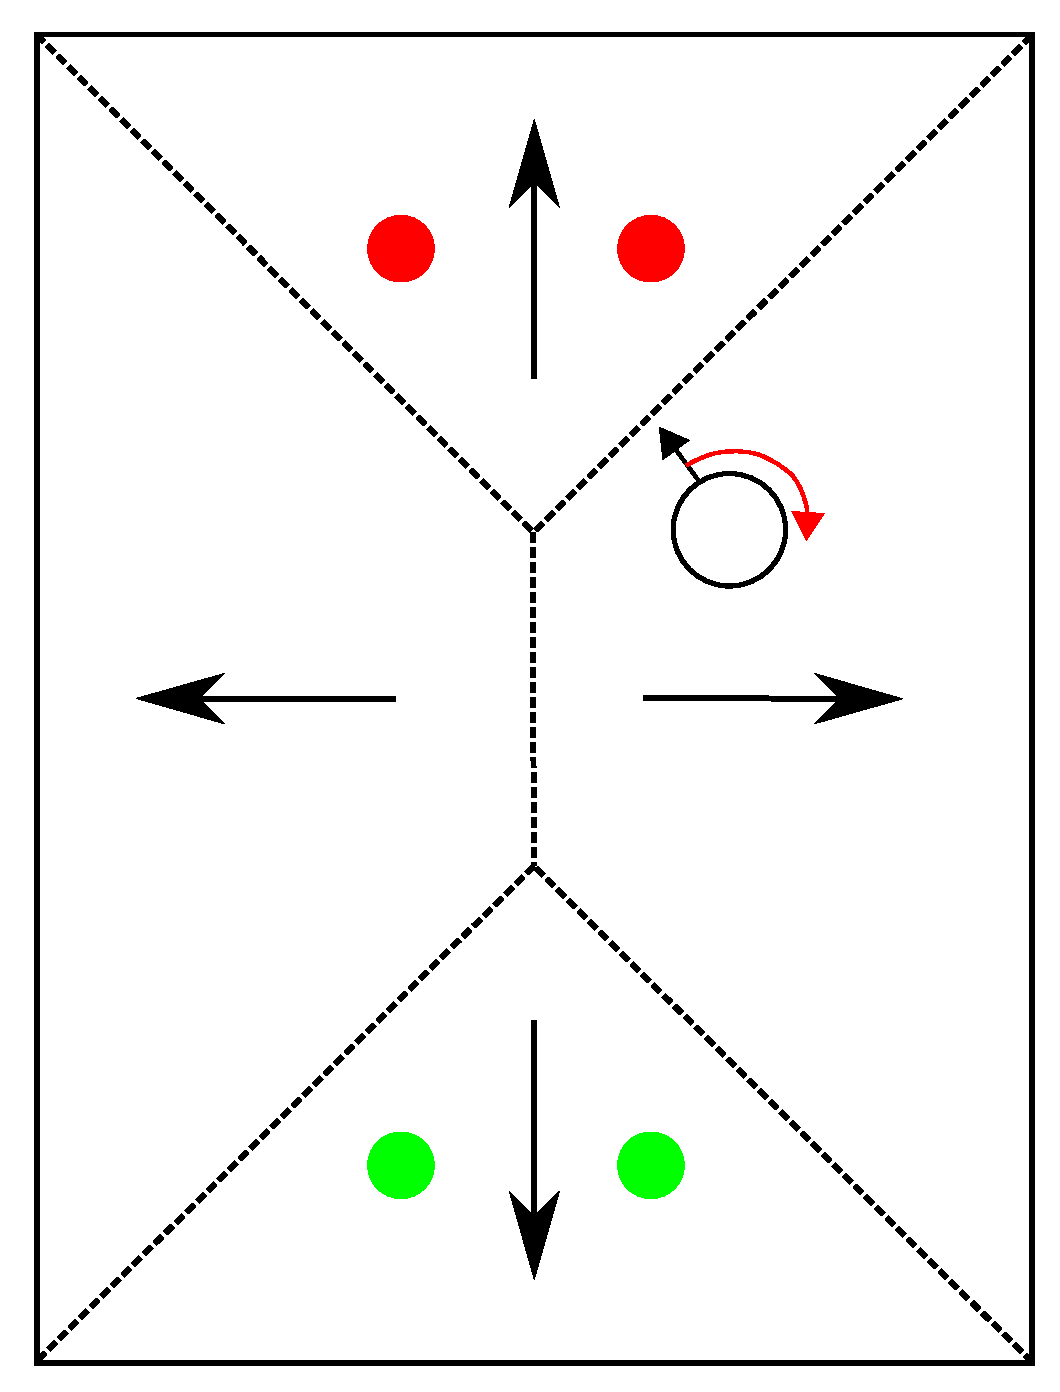
\includegraphics[scale=.4]{showcaseSplit.pdf} 	
		\caption{Gebietsaufteilung im Schaukasten}
		\label{fig:showcaseSplit}
	\end{center}
\end{figure}

\section[Finite-State-Machine des DiWheelDrive-Microcontrollers]{Finite-State-Machine des DiWheelDrive-Microcontrollers\hfill {\normalsize J.E. \& T.M.}} %TODO: Julian E. & Timo M.

Nachdem die Ladestation erfolgreich angefahren wurde, wird durch eine CAN-Nachricht dem DiWheelDrive-Board signalisiert, dass die weiteren Schritte des Einparkens eingeleitet werden sollen.
Auf dem Microcontroller wird eine State-Machine ausgeführt, die so lange im \textit{IDLE}-Zustand wartet, bis das Ladeverhalten angestoßen wird (siehe Abb. \ref{fig:uC_statmachine}).
Der nächste Zustand ist \textit{MOVE INTO STATION}, welcher in Kapitel \ref{kap:einparken_ladestation} erläutert wird. Ist dies erfolgreich abgeschlossen, so folgen die Zustände \textit{TURN AROUND} und \textit{ADJUST POSITION}, welche in Kapitel \ref{kap:andocken_ladestation} erklärt werden. Anschließend wird der Ladevorgang des AMiRos gestartet und überwacht. Dies geschieht in den Zuständen \textit{INITIATE CHARGING} und \textit{CHARGING}. Diese sind im Kapitel \ref{kap:ladevorgang} beschrieben.

Sollte ein Zustand nicht erfolgreich ausgeführt werden können, so gibt es definierte Routinen, die abermals ausgeführt werden müssen. Sollte die CAN-Nachricht für einen Abbruch des Ladevorganges eingehen, so wird dieser sofort unterbrochen und die State-Machine wird in den \textit{IDLE}-Zustand versetzt.

\begin{figure}[h]
	\begin{center}
		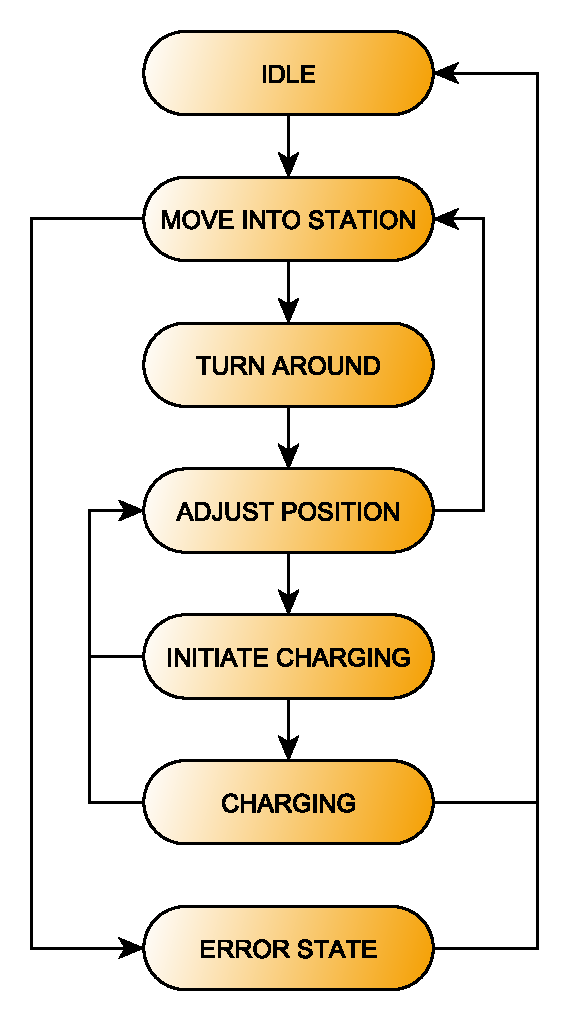
\includegraphics[width=0.4\textwidth]{uC_statemachine.pdf} 	
		\caption{Finite-State-Machine des DiWheelDrive-Microcontrollers}
		\label{fig:uC_statmachine}
	\end{center}
\end{figure}

\section[Einparken in der Ladestation]{Einparken in der Ladestation\hfill {\normalsize J.E.}}\label{kap:einparken_ladestation} %TODO: Julian E.
Dem Anfahren der Ladestation der Ladestation folgt das Einparken. Dieser Vorgang ist auf dem DiWheelDrive-Mikrocontroller implementiert, um eine Unabhängigkeit von optionalen Komponenten, wie dem Cognition-Board des AMiRo, herzustellen. Das Ziel des Einparkens in die Ladestation ist es, dass sich der AMiRo bündig in der ``Bucht'' der Ladestation (siehe Abb. \ref{fig:einparken}) befindet. Am Ende dieses Vorgangs ist der AMiRo so ausgerichtet, dass er der Ladestation zugewandt ist.

\subsection[Vermessung des Magnetometers]{Vermessung des Magnetometers\hfill {\normalsize J.E.}}
Im Rahmen dieses Projektes wurde das Magnetometer des AMiRo untersucht, um festzustellen, ob es zum Detektieren der Ladestation und anschließendem Einparken geeignet ist.
Bei dem Magnetometer handelt es ich um das HMC5883L-Board von Honeywell.
Die Messreihen wurden wie folgt angefertigt. Der AMiRo wurde mit der Vorderseite nach Norden ausgerichtet. Dies definieren wir als $0^\circ$. Nun beginnt der AMiRo eine Rotation in positiver Richtung. In etwa $10^\circ$-Abständen werden die Sonsordaten des Magnetometers erfasst und ausgegeben. Das Magnetometer verfügt über drei Achsen. Die magnetische Flussdichte entlang der Achsen ist über eine Schnittstelle des DiWheelDrive in $\mu$Gauss abrufbar. Der Verlauf einer solchen Messung ist in \ref{fig:no-station} zu sehen.
Grafik \ref{fig:station-2-90} zeigt die Messdaten für die Situation, in der sich die Ladestation etwa zwei Zentimeter und $90^\circ$ von der Ausgangsposition des AMiRos befindet.
Abbildung \ref{fig:station-0-90} stellt dar, dass es zu maximal negativen Messdaten kommen kann, wenn sich der AMiRo direkt an der Station befindet. Dies kann umgangen werden, indem maximal negative Messwerte als maximal positive angesehen werden.

Solche Messreihen wurden für verschiedene Abstände und Positionen der Ladestation aufgenommen. Das Resultat dieser Messungen ist, dass die Ladestation nur innerhalb von ein bis zwei Zentimetern vom AMiRo erkennbar ist. Außerdem kann sie nur erkannt werden, wenn der AMiRo ihr zugewandt ist. Dies erklärt sich dadurch, dass das Magnetometer im vorderen Bereich des AMiRo verbaut ist. Ein Erkennen der Station im Vorbeifahren ist also nicht möglich.

Die Implementierung des Einparkens beschränkt sich auf die X-Achse des Magnetometers. Diese liefert einen maximalen Ausschlag, wenn der AMiRo der Ladestation zugewandt ist (siehe \ref{fig:station-2-90}). Die Z-Achse liefert lediglich einen kleinen Ausschlag. Die magnetische Flussdichte der Y-Achse verläuft im Umfeld des Winkels der Ladestation von einem maximal positiven Wert zu einem maximal negativen Wert. Dieser Nulldurchgang ist schwieriger zu detektieren.

% Negative Werte
% herausrechnen -> Tagesabhängig
% Dies ist bedingt durch die ... mit Hilfe des Magnetometers. Deswegen AMiRo vorfährts einparken
%TODO: Magnetometer und Station genauer beschreiben, Bezug auf x-Achse
% Detektion nicht im vorbeifahren möglich
% Magnet vorne, auch nur vorne mag Flussdichte messbar
% Kurvenverlauf für Achsen
%TODO: Magnetometer-Typ

\begin{figure}
	\subfigure[]{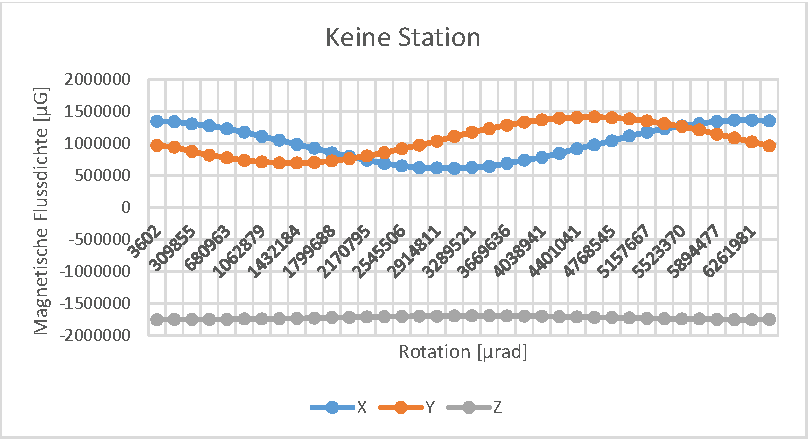
\includegraphics[width=0.7\textwidth]{no-station.pdf}\label{fig:no-station}}
	\subfigure[]{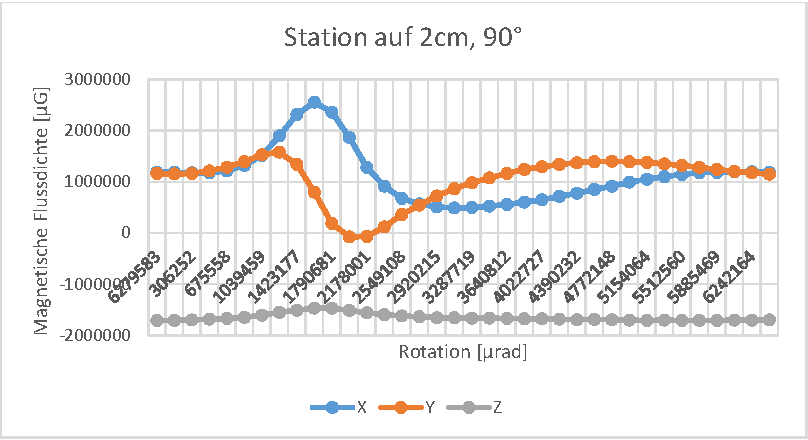
\includegraphics[width=0.7\textwidth]{station-2-90.pdf}\label{fig:station-2-90}}
	\subfigure[]{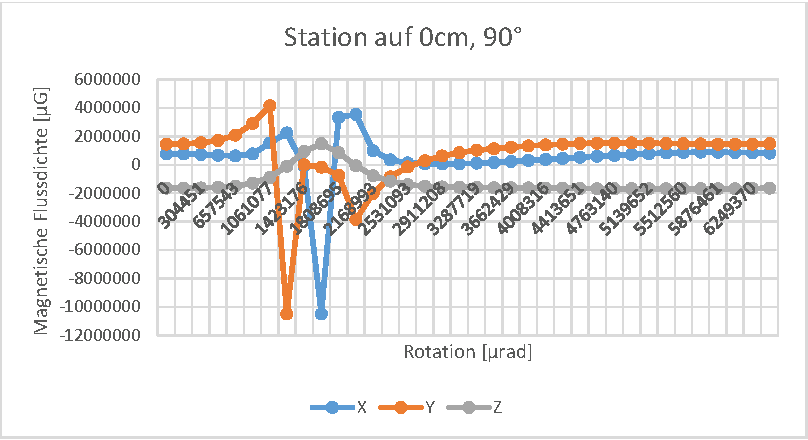
\includegraphics[width=0.7\textwidth]{station-0-90.pdf}\label{fig:station-0-90}} 
	\caption{Visualisierung der Messdaten}
	\label{fig:messdaten}
\end{figure}

\subsection[Ablauf des Einparkens]{Ablauf des Einparkens\hfill {\normalsize J.E.}}
In der angenommenen Ausgangssituation befindet sich der AMiRo in einem Abstand von ein bis zwei Zentimetern vom Magneten der Ladestation. Nun wird ein globaler Scan mit Hilfe des Magnetometers durchgeführt, d.h. der AMiRo dreht sich um die eigene Achse und nimmt währenddessen kontinuierlich Werte mit dem Magnetometer auf. Der Winkel, unter dem der maximale Sensorwert des Magnetometers gemessen wurde, wird gespeichert. Wurde eine vollständige $360^\circ$ Drehung abgeschlossen, richtet sich der AMiRo zu dem Winkel aus, unter dem der maximale Ausschlag des Magnetometers gemessen wurde. Anschließend beginnt eine Vorfährtstrajektorie bis ein Hindernis erkannt wurde. Die Hinderniserkennung erfolgt mit Hilfe der Infrarot-Ringsensoren und der Odometrie. Die reine Hinderniserkennung nur mit Hilfe der Ringsensoren ist problematisch, da die Ladestation mit schwarzen Klebestreifen versehen ist, die durch die Infrarotsensoren kaum erkennbar sind.

%TODO: mehr zu Odometrie

Nachdem ein Hindernis, beziehungsweise die Ladestation, erreicht wurde, werden die vorderen Ringsensoren überprüft. Liefern diese einen Maximalwert, so wurde die Station erreicht und das Einparken in die Ladestation war erfolgreich. %TODO: welche Sensoren
Ist dies jedoch nicht der Fall, so ist ein Korrekturschritt nötig (vgl. \ref{fig:einparken}).
Um festzustellen in welche Richtung die Trajektorie versetzt werden muss, wird ermittelt, ob sich der AMiRo auf der rechten oder linken Seite der Bucht befindet. Dies wird wiederum mit Hilfe des Magnetometers bestimmt. Zunächst wird eine Rotation nach Links vorgenommen und es wird die magnetische Flussdichte gemessen. Danach wird die vorherige Rotation rückgängig gemacht und eine Rotation nach Rechts im selben Winkel ausgeführt. Es wird ebenfalls die magnetische Flussdichte gemessen und zur Ausgangsposition zurück rotiert. Nun werden diese beiden Werte mit einander verglichen. Ist der Wert der linken Messung größer als der, der rechten, so muss sich der AMiRo links von der Einbuchtung befinden. Dies gilt analog im umgekehrten Fall.

Nun kann der Korrekturschritt vollzogen werden. Es folgt eine $90^\circ$-Rotation gemäß der Korrekturrichtung, eine kurze Vorfährtstrajektorie und eine Rückrotation um $90^\circ$ entgegengesetzt der Korrekturrichtung. Somit wurde die Trajektorie versetzt. Nun wird beginnt wiedermals eine Vorfährttrajektorie bis ein Hindernis erkannt wurde. Dieses Verhalten wird insgesamt dreimal wiederholt. Wurde bis dahin die Ladestation nicht erreicht, so wird die Kontrolle an die höhere Logik übergeben.

Während der Ermittlung des Korrekturrichtung und der Korrektur ist es möglich, dass der AMiRo bereits die Zielposition erreicht hat. Dies ist darauf zurückzuführen, dass die vordere Gehäuseschraube des AMiRo vom Magneten der Ladestation angezogen wird. Deswegen werden zwischen den einzelnen Schritten immer wieder die Ringsensoren überprüft und ermittelt, ob diese bereits einen maximalen Ausschlag liefern.

\begin{figure} []
	\subfigure[Ladestation]{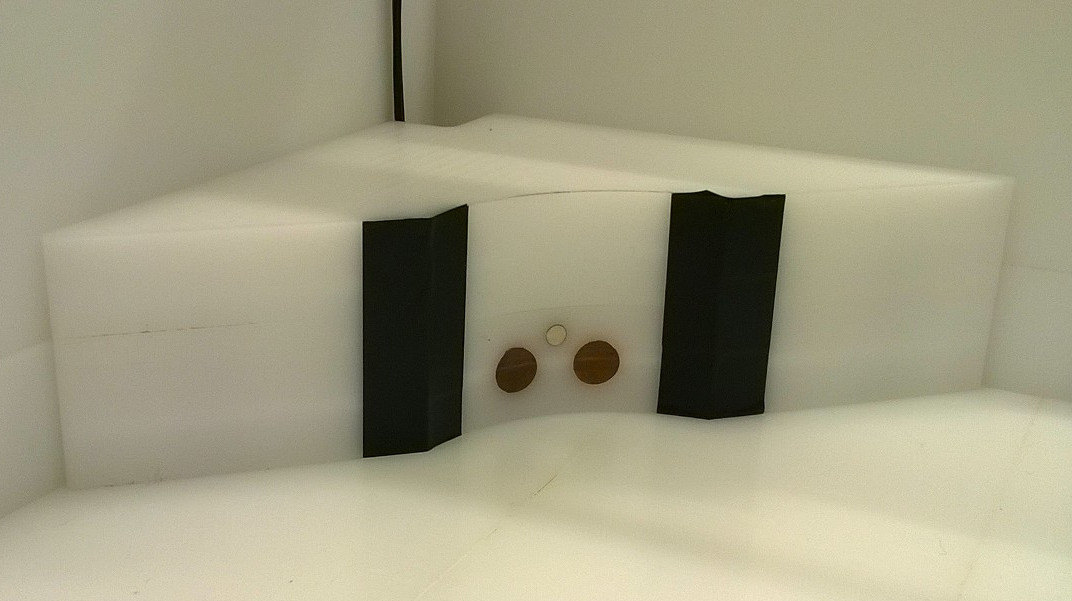
\includegraphics[width=0.45\textwidth]{Ladestation-croped.jpeg}\label{fig:ladestation}} 
	\subfigure[Einparken]{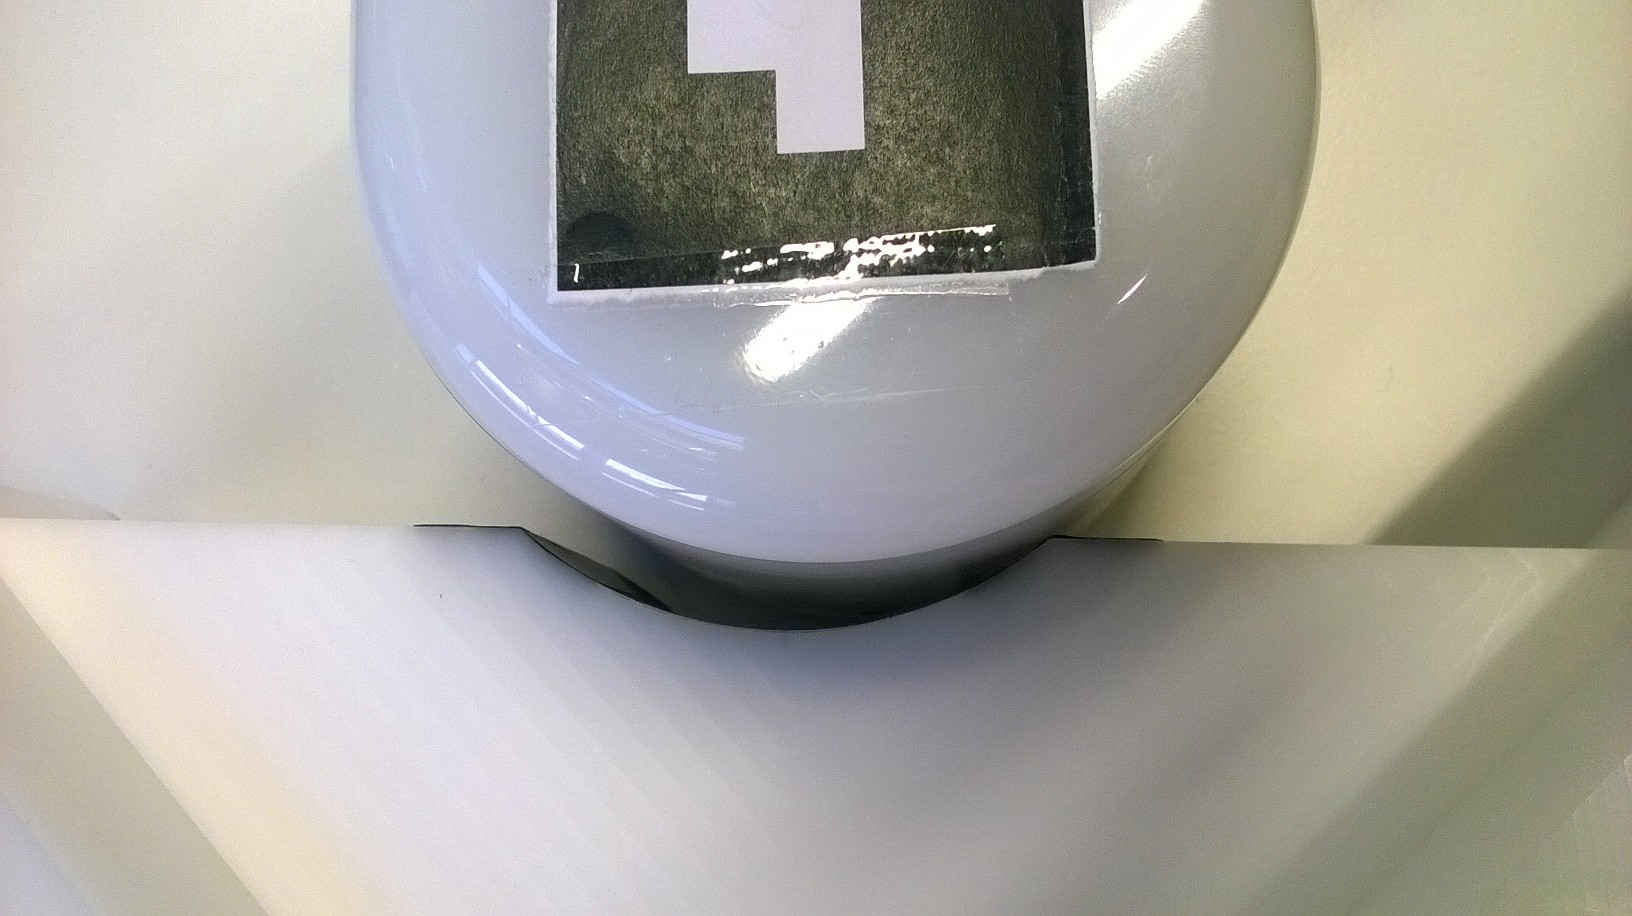
\includegraphics[width=0.45\textwidth]{Einparken.jpeg}\label{fig:einparken}} 
	\caption[Ladestation und Einparken]{Bild (a) zeigt die Ladestation mit der Einbuchtung, den zwei Kontakten, sowie dem Magneten in der Mitte. Bild (b) zeigt einen fehlgeschlagenen Einparkversuch, der einen Korrekturschritt benötigt.}
	\label{fig:ladestation-einparken}
\end{figure}

\section[Andocken an die Ladestation]{Andocken an die Ladestation\hfill {\normalsize T.M.}}\label{kap:andocken_ladestation} %TODO: Timo M.
Nachdem der AMiRo erfolgreich in der Ladestation eingeparkt ist werden anschließend die Ladepins auf der Rückseite des Roboters zu den Ladekontakten der Station ausgerichtet. Dabei ist es notwendig, dass alle Pins die Kontakte berühren, da es bei Stromspitzen sonst zu Schäden am AMiRo kommen könnte.

Als ersten Schritt wird zunächst eine 180$^\circ$ Drehung durchgeführt, durch die der AMiRo grob in die Ladeposition gedreht wird. Die Drehung wird anhand der Odometriedaten des Roboters durchgeführt. Dabei kann eine gewünschte Fehlertoleranz als Argument übergeben werden. Da eine exakte Drehung um 180$^\circ$ kompliziert ist, wird hier eine Fehlertoleranz von 5$^\circ$ eingeräumt, damit die Drehung schnell durchgeführt werden kann und der AMiRo nicht die Position mehrfach verbessern muss, bis exakt 180$^\circ$ erreicht sind. Diese Toleranz hat auf das anschließende Justieren der Position keine Auswirkungen.

Für die Justierung der Ladeposition des AMiRos werden die Daten der beiden hinteren Abstandssensoren genutzt. Um diese zur Ausrichtung des Roboters nutzen zu können, wurden an der Station zwei schwarze Streifen angebracht (siehe Abb. \ref{fig:charging_station}). Diese bieten einen hohen Kontrast für die UV-Sensoren im Vergleich zur weißen Station. So liefern die Sensoren den maximalen Wert von 0xFFFF, wenn sie sich direkt vor der weißen Ladestation befinden und einen im Vergleich sehr niedrigen Wert von unter 0x2000, wenn sie den Abstand zu einen schwarzen Klebestreifen messen. 
Die Klebestreifen sind so angebracht, dass sich beide hinteren Abstandssensoren genau vor einer weißen Fläche befinden, wenn die Ladeposition erreicht ist. 
Das heißt, dass die Position des AMiRos so lange justiert werden muss, bis beide Sensoren den Wert 0xFFFF liefern. 
Dafür werden die Werte der Abstandssensoren ausgelesen und anhand dieser wird nun unterschieden in welcher Position sich der AMiRo befindet und welches der nächste Schritt ist, um die Ladeposition zu erreichen. 

\begin{figure}[]
	\begin{center}
		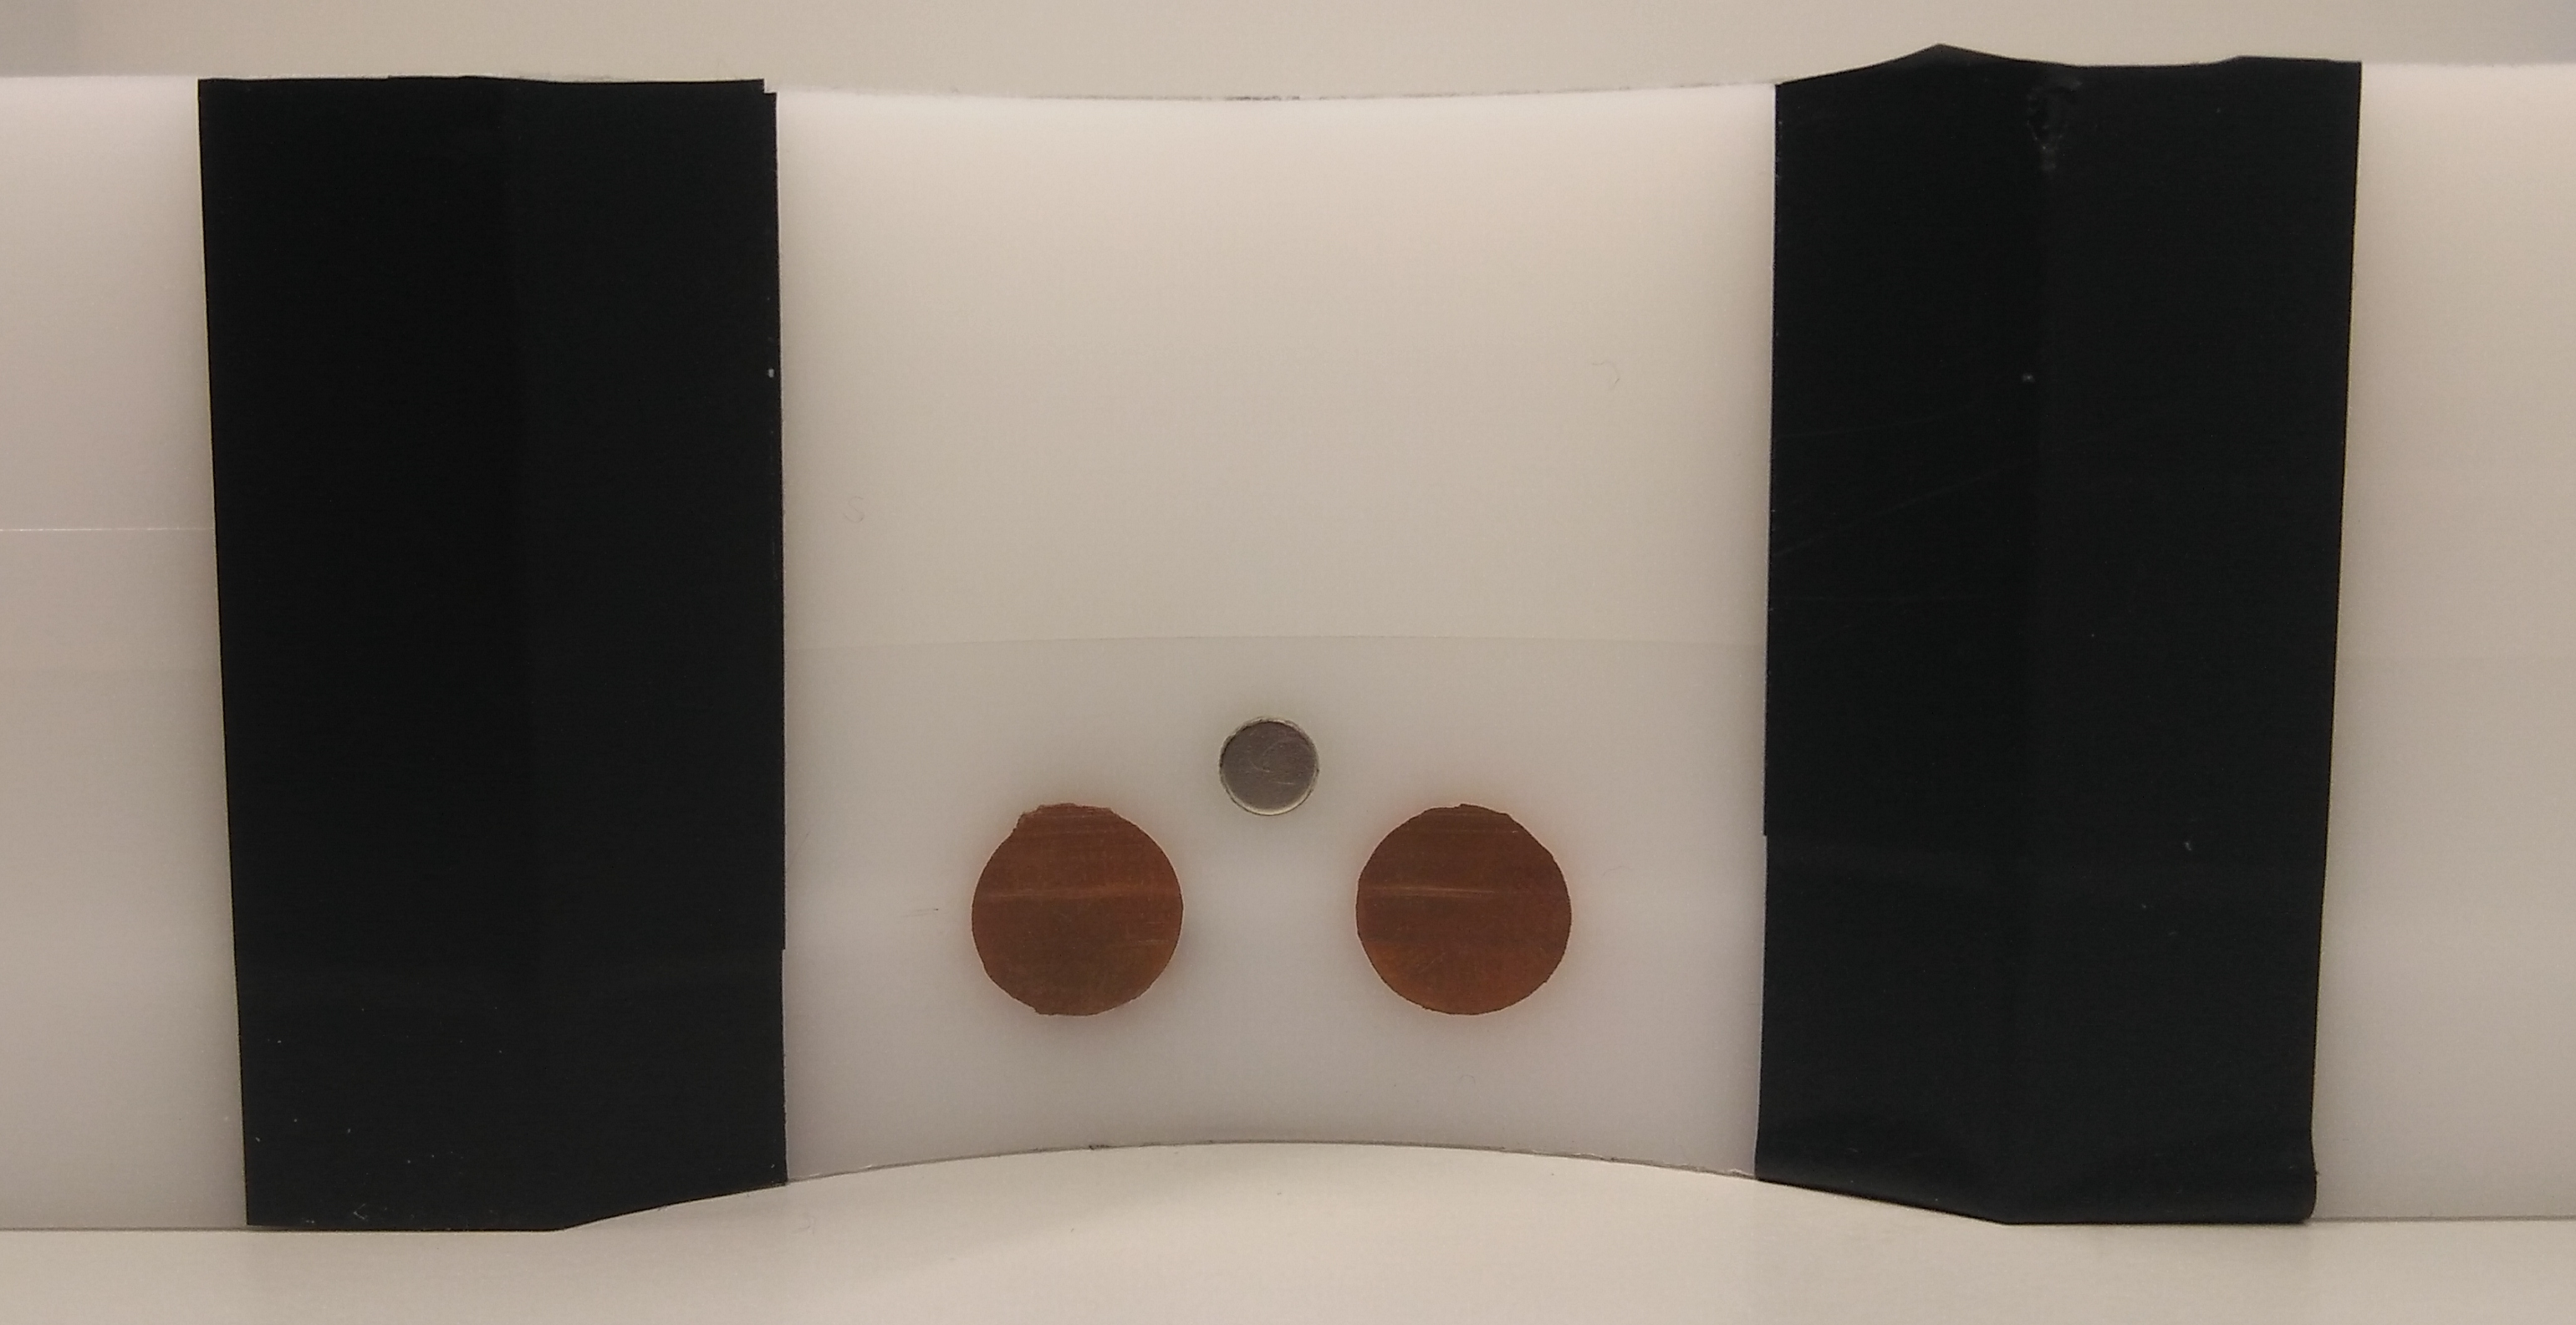
\includegraphics[width=0.6\textwidth]{charging_station_stripes.jpg} 	
		\caption{Ladestation mit Klebestreifen}
		\label{fig:charging_station}
	\end{center}
\end{figure}

Sollte einer der beiden Sensoren 0xFFFF als Wert liefern und der andere einen zu 0xFFFF abweichenden Wert, so steht der AMiRo direkt vor der Wand der Station, muss aber noch in die Richtung des Sensors mit vollem Ausschlag gedreht werden. Da der Magnet der Station eine hohe Anziehung auf die hintere Befestigungsschraube des AMiRos ausübt, ist es nicht möglich den Roboter durch minimales Ansteuern der PWM\footnote{Pulsweitenmodulation}-Steuerung der Motoren zu drehen. Deshalb fährt der Roboter ein kleines Stück aus der Station heraus um sich anschließend in die gegebene Richtung in die Station hinein zu bewegen. 
Wenn ein Sensor einen Wert über 0x4000 und der andere unter 0x4000 liefert, bedeutet dies, dass sich der AMiRo mit einem Abstand vor der Station befindet und seine Position außerdem ein wenig verdreht ist. In dieser Situation muss sich der Roboter in die Richtung des Sensors mit höherem Wert drehen und sich auf die Station zu bewegen. 
Geben beide Sensoren einen Wert über 0x4000 aus, so steht der AMiRo mit Abstand zur Station, muss jedoch nicht gedreht werden. In diesem Fall wird eine gerade Bewegung in Richtung der Station ausgeführt. 
Sollten beiden Sensoren einen Wert unter 0x4000 liefern, so steht der AMiRo in einem zu hohen Abstand zur Ladestation und das Einparken in die Ladestation wird nochmals eingeleitet.

Bevor der Ladevorgang eingeleitet wird, wird die Position des AMiRos nochmals überprüft. Hierfür werden die aktuellen Odometriedaten des Roboters abgerufen und gespeichert. Anschließend wird die PWM-Steuerung der Motoren deaktiviert, was zur Folge hat, dass sich die Reifen frei drehen können. Sollte der AMiRo noch nicht korrekt zur Ladestation ausgerichtet sein, kann die Position des Roboters durch die Wirkung des Magneten auf die Befestigungsschraube verändert werden. Dabei werden die aktuellen Odometriewerte mit den gespeicherten abgeglichen. Sollte sich nach einer Sekunde keine Änderung der Position ergeben haben, so wird eine korrekte Ladeposition angenommen und der Ladevorgang gestartet. Sollte sich die Odometrie verändern, so wird das Justieren nochmals eingeleitet. 




%- Ausgangssituation: AMiRo steht vorwärts in der Ladestation
%- 180$^\circ$ Drehung anhand der Odometrie um die Ladepins zur Station zu richten
%- Justierung der Position anhand der Abstandssensoren und der schwarzen Streifen
%- Abschalten der PWM und Überwachung, ob sich die Position ändert 
%	- Mögliche Fehlerquellen für Positionsänderung: 
%		- AMiRo wird durch den Einfluss des Magnetfeldes auf die Schraube gedreht, da die Position noch nicht gut genug justiert ist
%		- AMiRo wird durch die Federung der Ladepins von der Station abgestoßen, da die Schraube nicht genau vor dem Magneten war und somit die magnetische Kraft nicht groß genug war 

\section[Ansteuern und Überwachen des Ladevorgangs]{Ansteuern und Überwachen des Ladevorgangs\hfill {\normalsize T.M.}}\label{kap:ladevorgang} %TODO: Timo M.

Sobald der AMiRo mit seinen Ladepins zu den Ladekontakten der Ladestation ausgerichtet ist, kann der Ladevorgang eingeleitet werden.
Zunächst wird dem PowerManagement-Board signalisiert, dass der DiWheelDrive-Ladepfad aktiviert werden soll. Nun wird kontrolliert, ob wirklich mindestens 9V an den Pins anliegen und die Akkus aufgeladen werden. Hierfür wird eine kurze Zeit gewartet, da es aufgrund von Signalfilterungen bei der Ermittlung der anliegenden Spannung zu Verzögerungen kommt. Sollten anschließend keine 9V anliegen und die Akkus nicht geladen werden, so wird der Ladevorgang abgebrochen und die Position des AMiRos zur Station wird nochmals justiert.
Liegt die Spannung an und die Akkus werden geladen, so wird während des Ladevorgangs der Status mittels LEDs visualisiert (siehe Abb. \ref{fig:amiro_charging}). 
Währenddessen wird außerdem auf die Odometriedaten des AMiRos geachtet, denn sollte sich etwas an der Position des Roboters ändern, ist nicht mehr sichergestellt, dass alle Pins die Ladekontakte berühren und der Ladevorgang wird abgebrochen. Ein Grund hierfür könnten äußere Einwirkungen wie ein Wackeln am Schaukasten sein.

Nachdem die Akkus des AMiRos voll geladen sind wird der DiWheelDrive-Ladepfad deaktiviert, die PWM-Steuerung aktiviert und der Roboter fährt ein Stück aus der Ladestation heraus.

\begin{figure}[]
	\begin{center}
		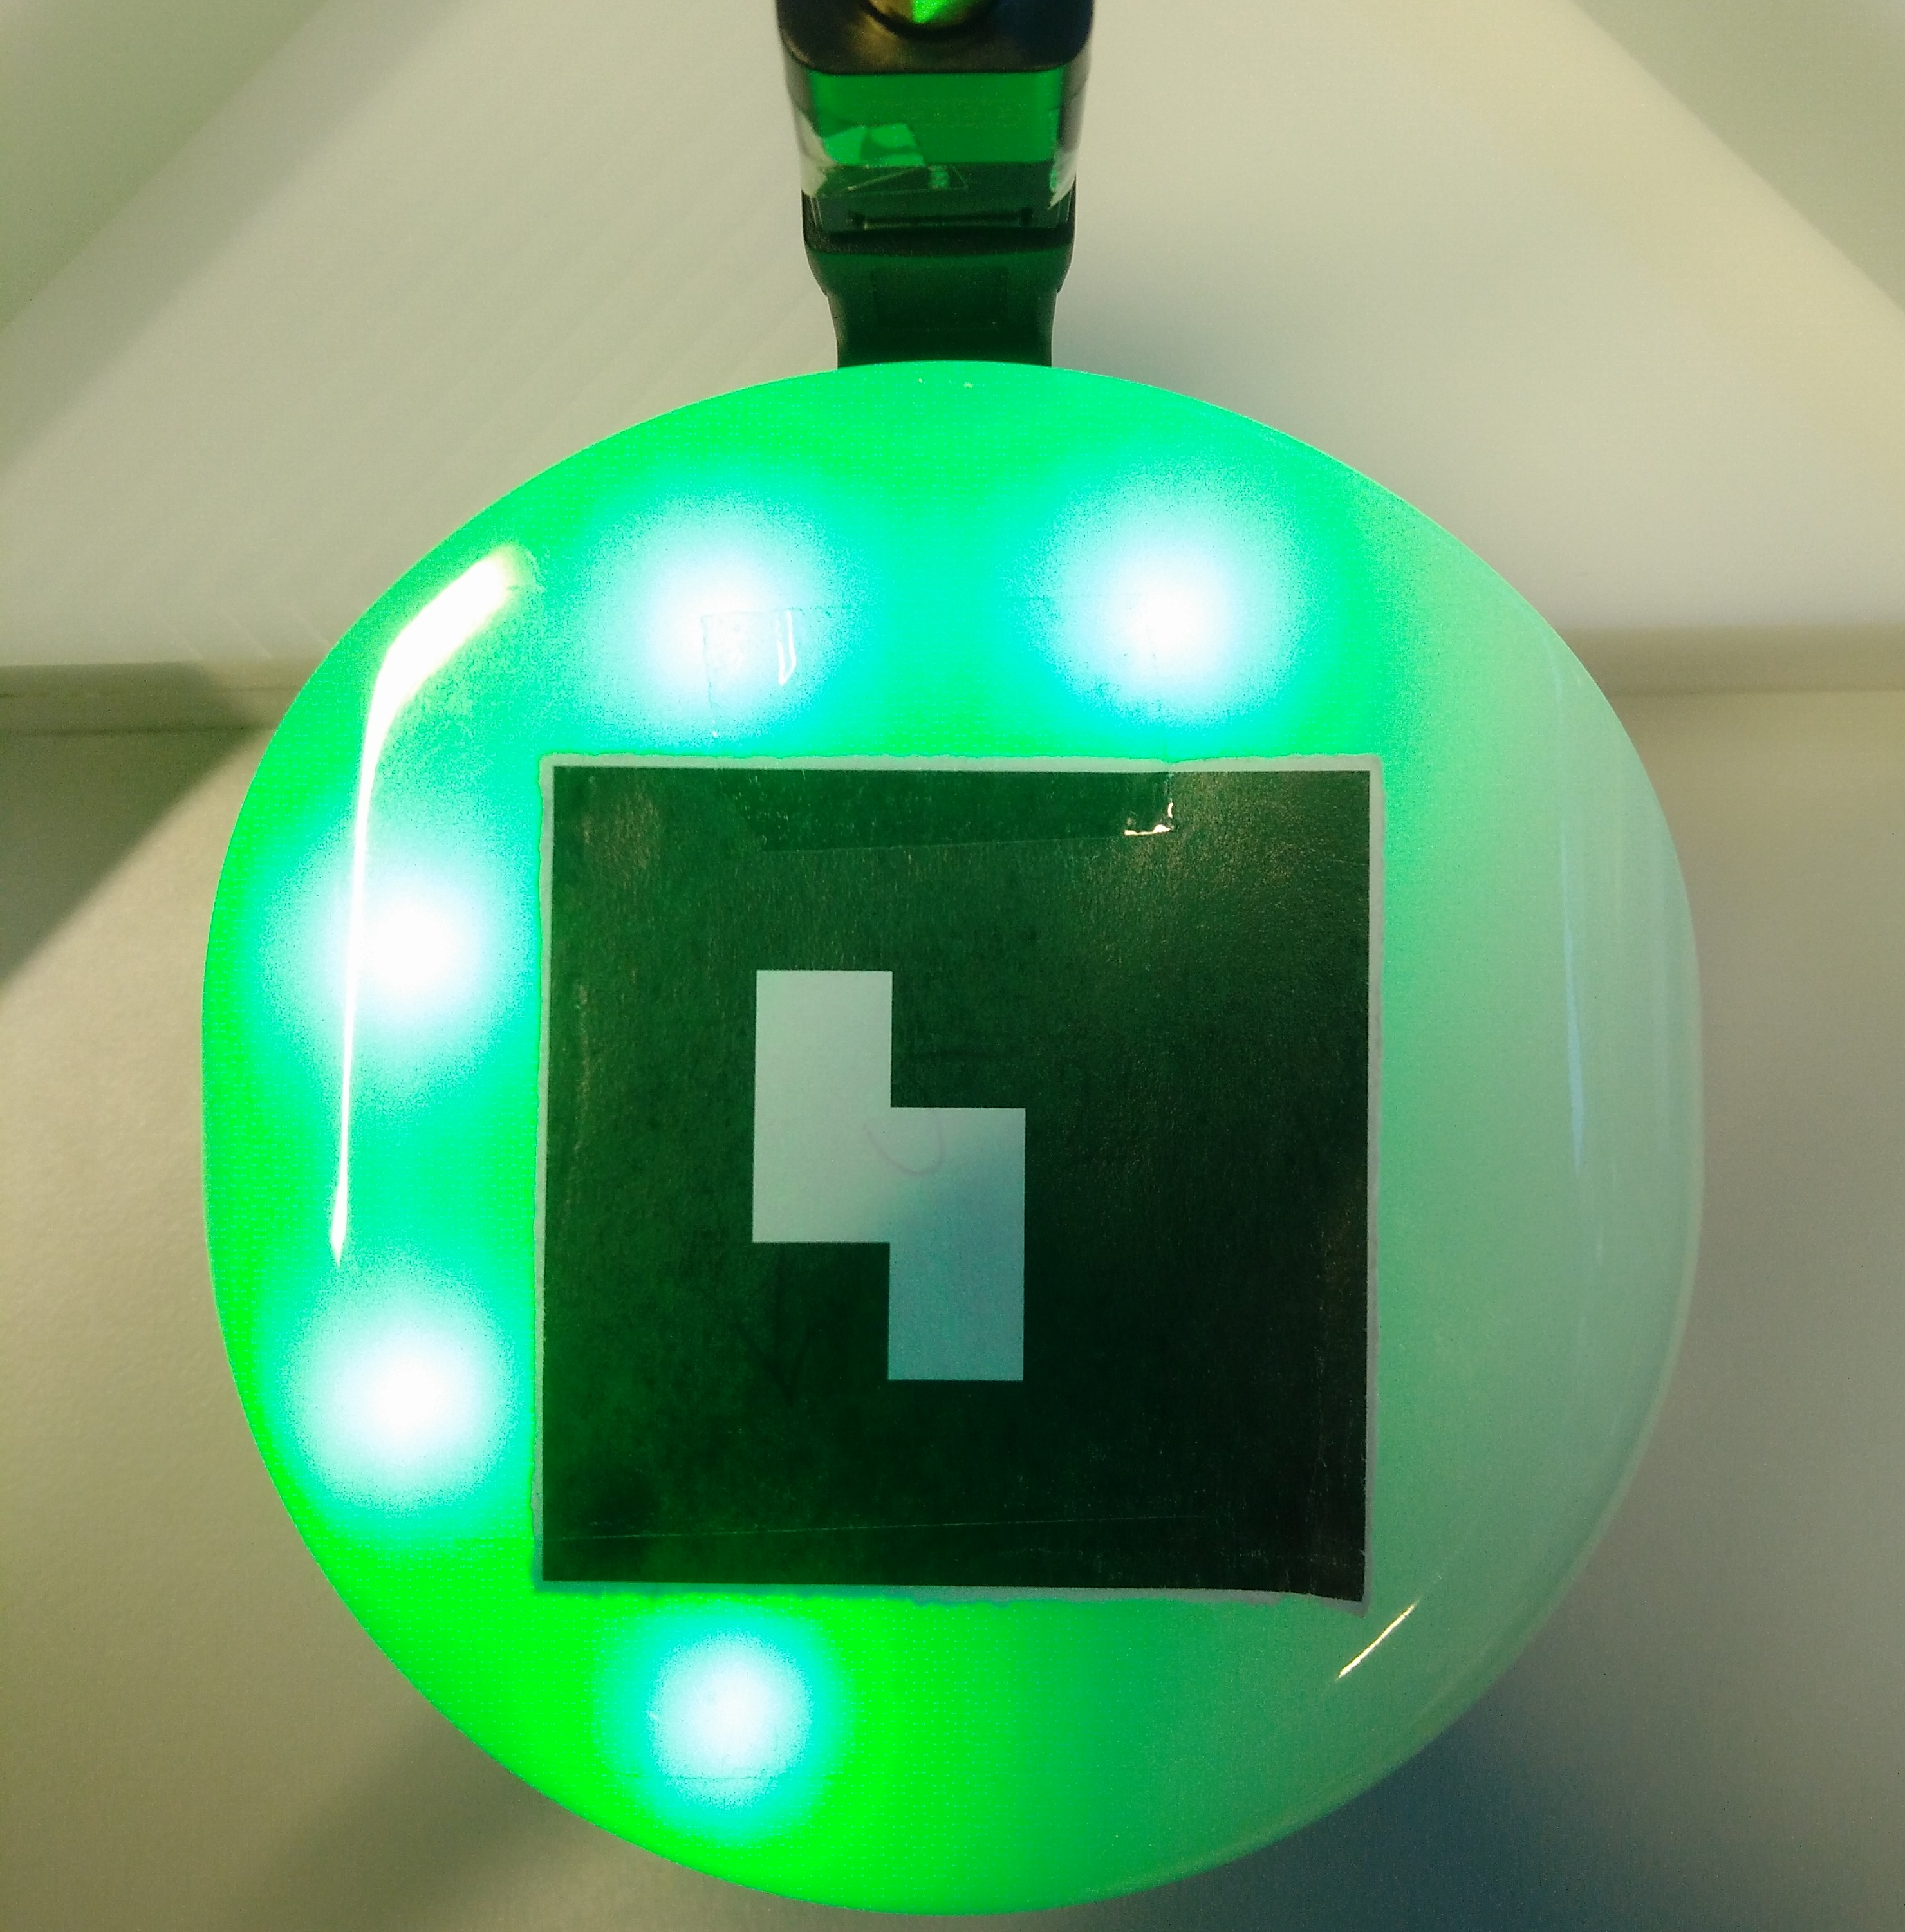
\includegraphics[width=0.5\textwidth]{AMiRo_charging.jpg} 	
		\caption{Ladeanimation}
		\label{fig:amiro_charging}
	\end{center}
\end{figure}



%- Aktivieren des DiWheelDrive-Board Ladepfades (+ kurzes Abwarten)
%- Kontrolle, ob mehr als 9V anliegen (wenn nicht -> Position erneut justieren)
%- Überwachen des Ladevorgangs
%	- Auslesen der Ladestatus der Akkus (\% und Zeit bis geladen)
%	- Überwachen der Odometrie 
%		- falls sich der AMiRo aufgrund von äußeren Einwirkungen bewegen sollte -> Abbruch des Ladevorgangs und Position erneut justieren
